\documentclass{standalone}
\usepackage{tikz}
\usetikzlibrary{arrows,shapes,positioning,shadows,trees}

\begin{document}
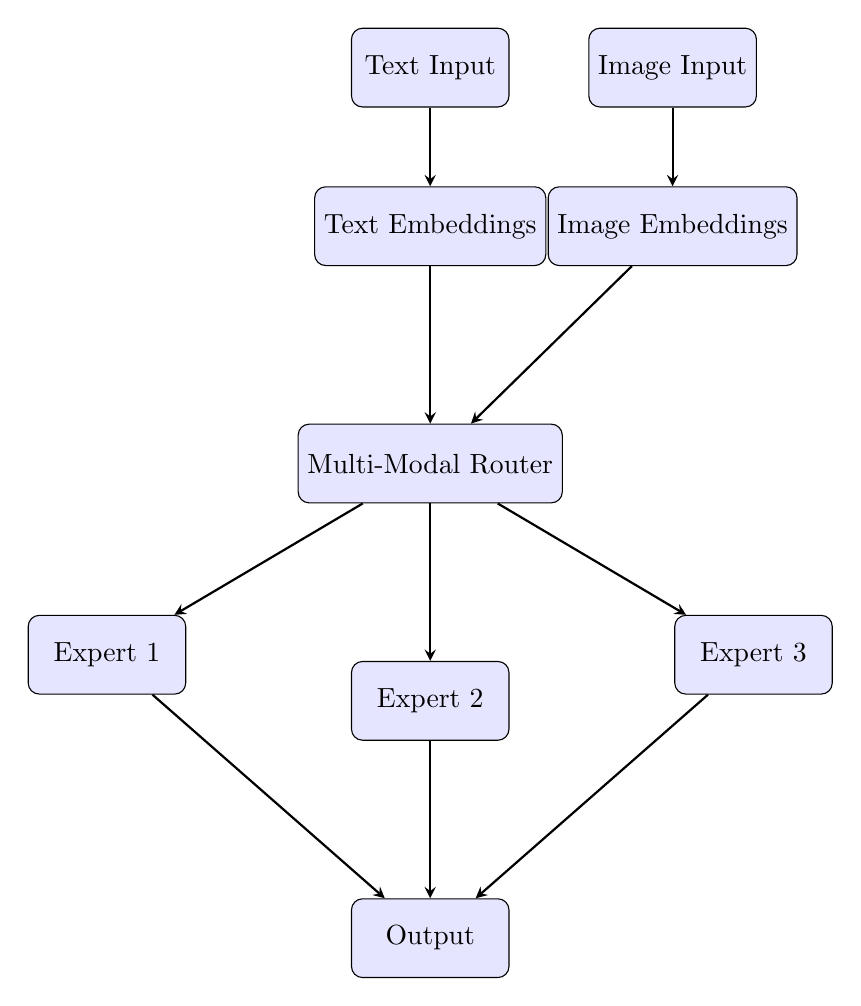
\begin{tikzpicture}[
    node distance = 1cm,
    box/.style={rectangle,draw,rounded corners,fill=blue!10,minimum width=2cm,minimum height=1cm},
    arrow/.style={->,>=stealth,thick}
]

% Input layers
\node[box] (text) {Text Input};
\node[box, right=of text] (image) {Image Input};

% Embedding layers
\node[box, below=of text] (text_emb) {Text Embeddings};
\node[box, below=of image] (image_emb) {Image Embeddings};

% Routing layer
\node[box, below=2cm of text_emb] (router) {Multi-Modal Router};

% Expert layers
\node[box, below left=2cm of router] (expert1) {Expert 1};
\node[box, below=2cm of router] (expert2) {Expert 2};
\node[box, below right=2cm of router] (expert3) {Expert 3};

% Output layer
\node[box, below=2cm of expert2] (output) {Output};

% Connections
\draw[arrow] (text) -- (text_emb);
\draw[arrow] (image) -- (image_emb);
\draw[arrow] (text_emb) -- (router);
\draw[arrow] (image_emb) -- (router);
\draw[arrow] (router) -- (expert1);
\draw[arrow] (router) -- (expert2);
\draw[arrow] (router) -- (expert3);
\draw[arrow] (expert1) -- (output);
\draw[arrow] (expert2) -- (output);
\draw[arrow] (expert3) -- (output);

\end{tikzpicture}
\end{document}
